Ich habe keine Ahnung wie der Christian bei dem konstanten Lärm- nicht nur Geräuschpegel, Lärmpegel ohne Ohrenstöpsel überhaupt ein Auge zumachen konnte.
Vielleicht trug das griechische Abendessen seinen Teil dazu bei, aber ausgeschlafen und fit sieht ganz anders aus.
Wir sind dann erstmal zum Walmart, um - zusammengefasst - Schrott zu kaufen.
Wasser war auch dabei sowie unser Frühstück bestehend aus Toastbrot und Käse, aber alles andere war nur Schrott.
Die Kekse mit Schokostücken, wie es sie bei uns auch gibt, waren noch okay, der 5Gum-Kaugummi mit Geschmacksrichtung Peppermint schmeckt nach Zahnarz und die Schnüre waren ungenießbar.
Unsere anschließende Suche nach einem At\&t Geschäft verlief erfolglos und so fuhren wir ohne Möglichkeit online zu buchen richtung \TOWN{San Diego}.
Auf dem Weg dahin standen nicht nur ein paar Windräder sondern hunderte.
Diese waren nicht so groß wie zuhause, dafür dichter zusammengepackt.\\

%\newpage
%\thispagestyle{empty}
%\begin{tikzpicture}[remember picture, overlay]
%\node[inner sep=0pt] at (current page.center) {%
%	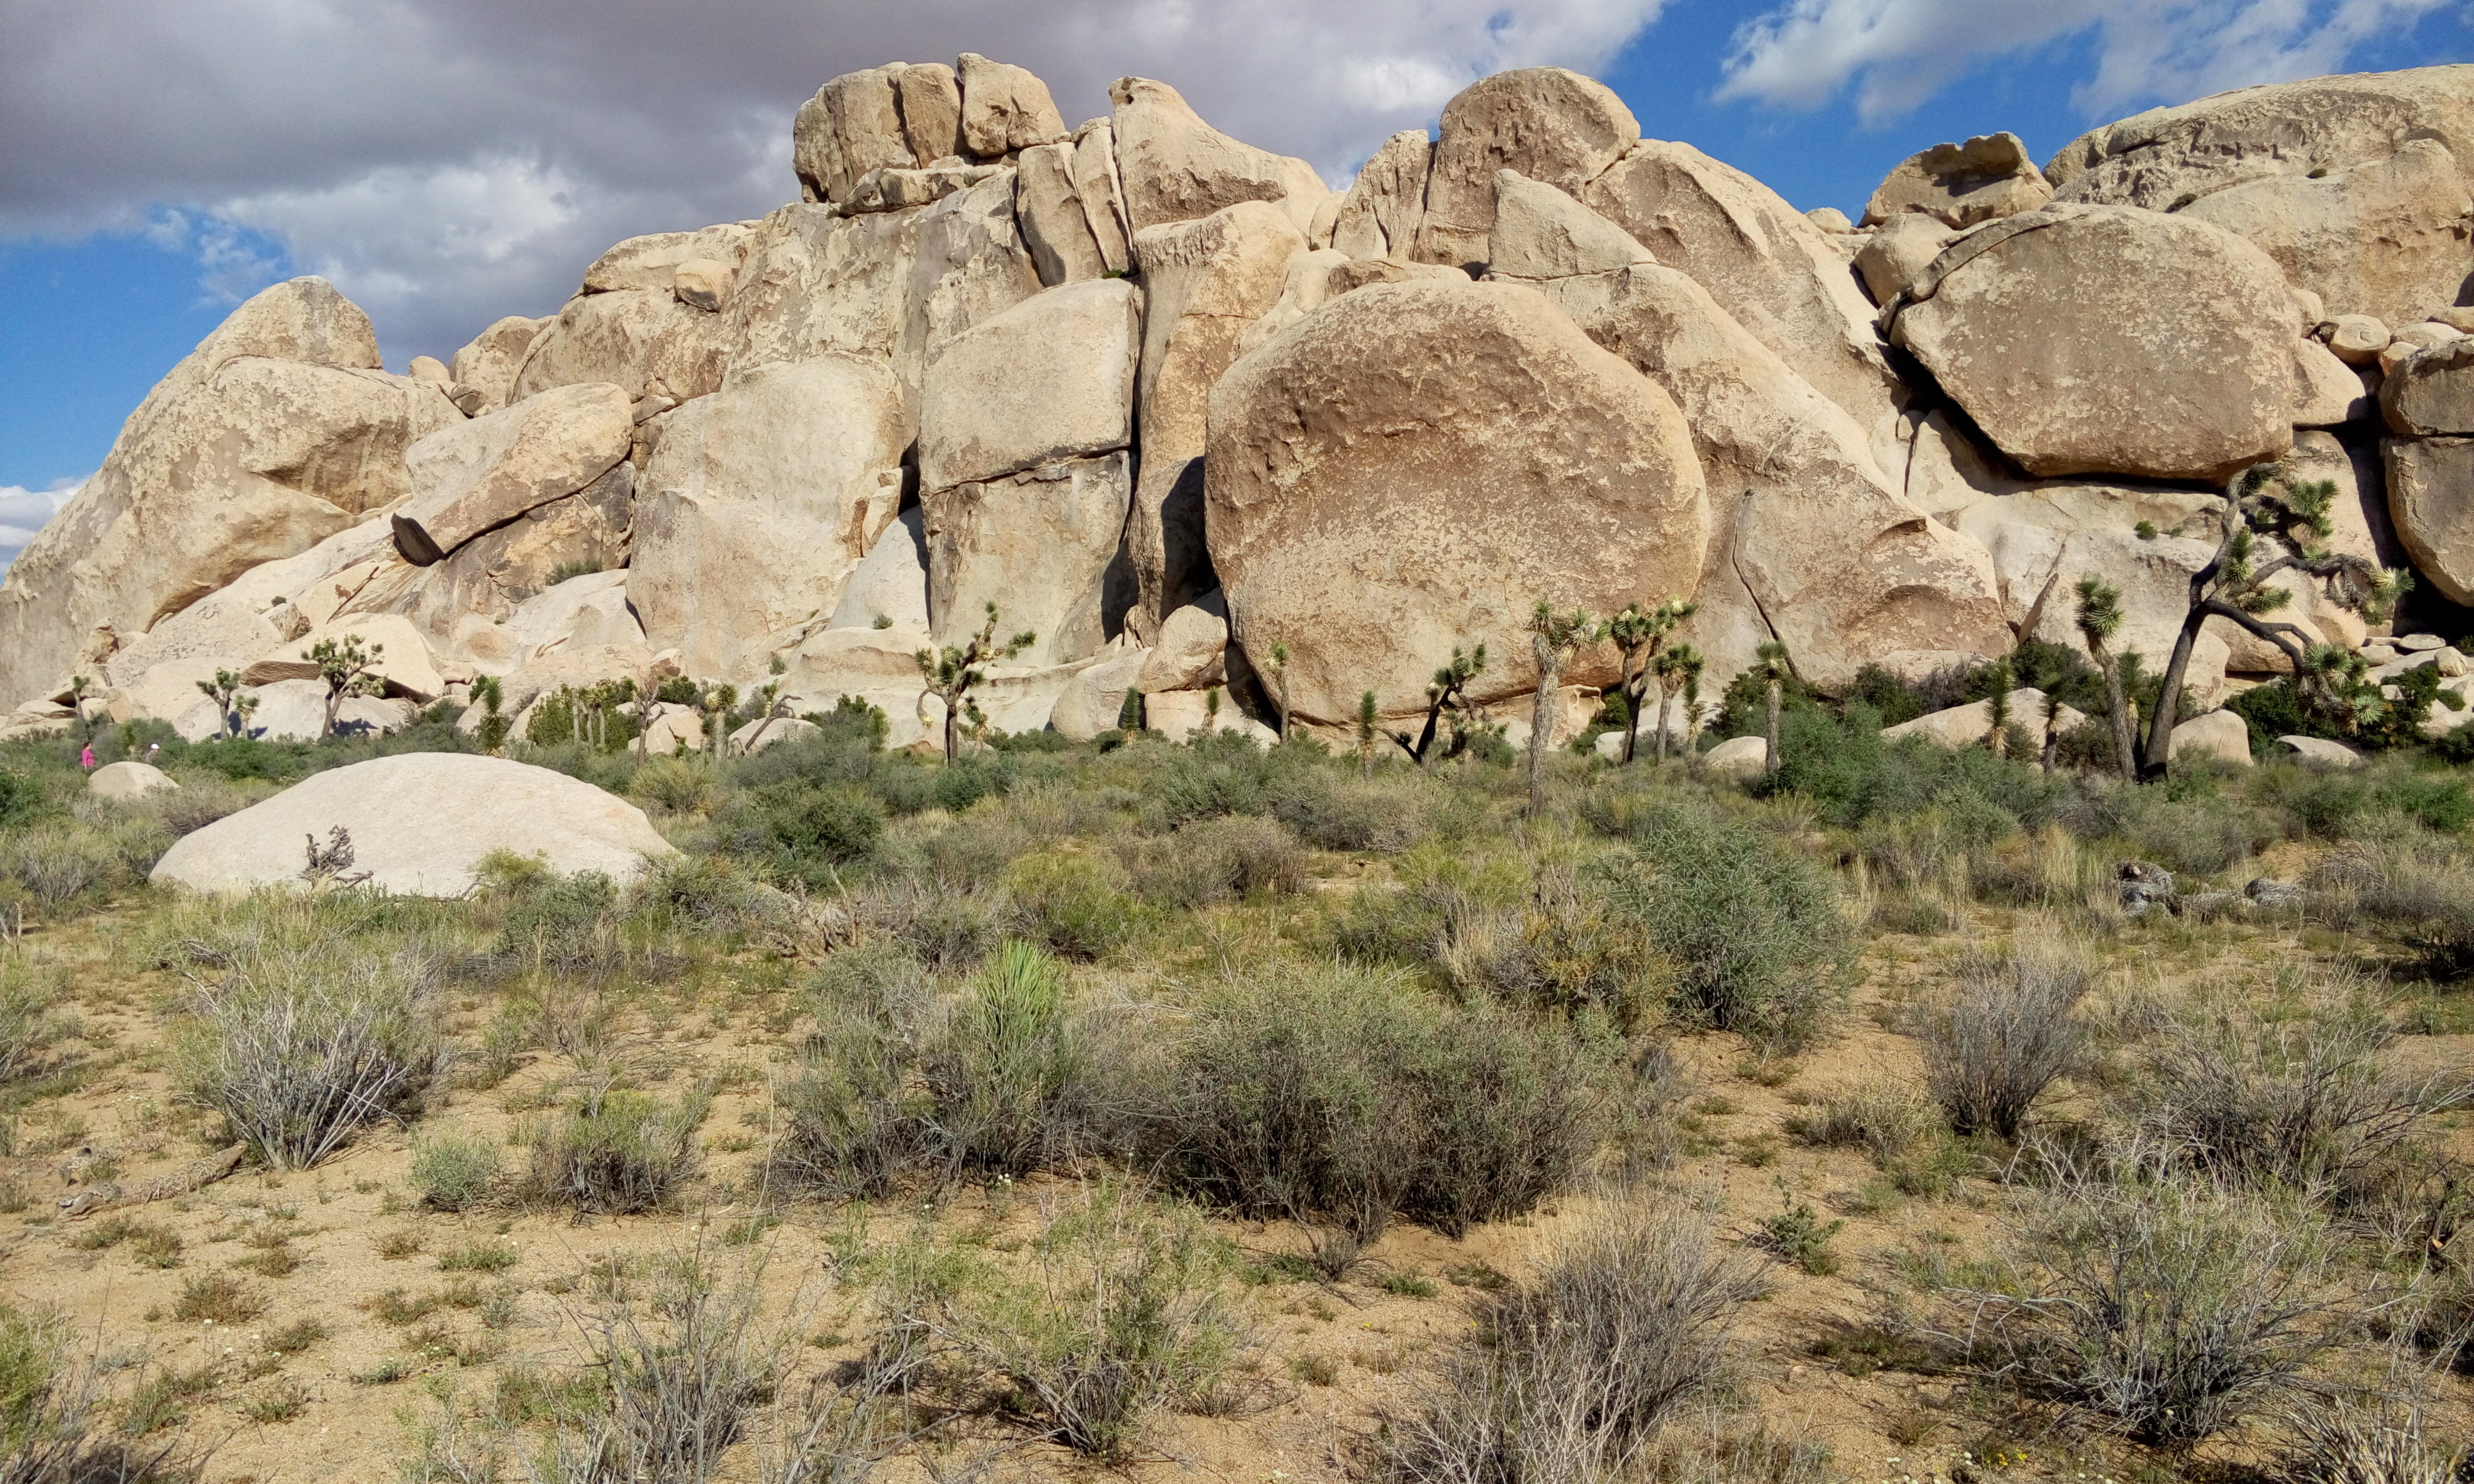
\includegraphics[width=\paperwidth,height=.5\paperheight]{12/image20160412_164403875.jpg};%
%};
%\end{tikzpicture}
%\newpage

Das letzte Stück bis San Diego auf dem sechs oder gar acht spurigen Freeway war dann alles andere als ein Zuckerschlecken.
Die Ansage des Navis \flqq Folgen Sie den linken Spuren\frqq \, stand unserem Wunsch möglichst rechts zu fahren, um die richtige Ausfahrt nicht zu verpassen, deutlich entgegen.
In den Hafen (\FOREIGN{Downtown}s) schafften wir es dann letztlich doch irgendwie und dort setzten wir nach einer kurzen Hafenbesichtigung unsere Suche nach einem At\&t Shop fort.
Gefunden haben wir auch einen, wir waren wieder online (Guthaben aufgeladen) und konnten uns so der Suche nach einer Unterkunft widmen.
Hotels gab es natürlich auch, doch das Hostel war deutlich günstiger, vor allem weil beim Hotel auch \textbf{kein} Parkplatz mit enthalten war.

%\thispagestyle{empty}
\begin{tikzpicture}[remember picture, overlay]
\node[inner sep=0pt] at (current page.center) {%
	\includegraphics[width=\paperwidth,height=.4\paperheight]{13/image20160413_183409144.jpg};%
};
\end{tikzpicture}

\vspace*{.4\paperheight}

Tagsüber stolperten wir im Hafen herum, am Abend wollten wir uns den \glqq berühmten\grqq \, Zoo bzw. das Drumherum anschauen.
Den Zoo haben wir nicht so recht ausmachen können, aber der Balboa Park in dem der Zoo eingebettet ist, ist selbst ganz schön.
Dieser befand sich mitten in der Einflugschneise des Flughafens.
Dort gab es auch ein Militärkrankenhaus sowie eine Schule.
Wo lernt es sich schließlich besser als in der Einflugschneise eines Flughafens?

Das Abendessen war dann nur flüssiger Natur, da die Küche kurz vorher geschlossen hatte.
